\documentclass{article}

\usepackage[shortlabels]{enumitem}
\usepackage[dvipsnames]{xcolor}

\definecolor{SkullKingBlack}{RGB}{30,30,30}
\definecolor{MermaidBlue}{RGB}{5,163,165}
\definecolor{PirateRed}{RGB}{216,48,48}
\definecolor{TreasureMap}{RGB}{98,71,135}

\usepackage{amsmath}
\usepackage{amssymb}

\usepackage{tikz}
\usetikzlibrary{positioning, shapes.geometric, decorations.pathreplacing, arrows.meta}

\usepackage{multirow}
\usepackage{hyperref}
\usepackage{subcaption}
\usepackage{float}

\newcommand{\Green}{\textcolor{LimeGreen}{Green}}
\newcommand{\Purple}{\textcolor{Orchid}{Purple}}
\newcommand{\Yellow}{\textcolor{Apricot}{Yellow}}
\newcommand{\Black}{Black}

\newcommand{\block}[2][\medskip]{#1\noindent\textbf{#2.}\ }

\renewcommand{\arraystretch}{1.25}

\title{\textsc{Skull King Rules}}
\author{Charles Kolozsvary}
\date{}

\begin{document}

\maketitle

\section*{Preface}
I've written this document to see if I have correctly learned all the rules and if I can simplify their explanation.
The official rule book can be found at \url{https://www.grandpabecksgames.com/pages/skull-king}. 

\section{The Name of the Game}
\textit{Skull King} is a ``trick taking'' card game.

\block{Trick}
A small period of play comprised of each player, one by one, playing a single card in clockwise order. At the end of each trick, at most one player is declared its winner. The winner gathers the cards just played and starts the next trick.

\block{Rounds}
The game consists of multiple rounds, and each round contains a number of tricks equal to how many cards were dealt for the round. 

\block{Common format}
Ten rounds are played in the game: one card is dealt in the first, two in the second, and so on.

\block{Goal}
The goal of the game is not to win as many tricks as possible. Rather, it is to \textit{accurately predict} how many tricks you will win each round.

\block{Bidding}
Before each round begins, players simultaneously declare the number of tricks they expect to win (their bid)
by raising as many fingers from a closed fist on the count of \textit{``Yo Ho Ho!''}

\block{Points and win condition}
Once all tricks are played for a round, players
earn points if their bid was correct and lose points if it was incorrect. Whoever has the most points after the agreed-upon number of
rounds is the winner.\footnote{If there is a tie, additional rounds are played until it is broken.}

\section{The Caaards}
\subsection{Suits}
There are four suits in the deck:\pagebreak
\begin{itemize}
\item \Green{} (parrot),
\item \Yellow{} (treasure chest), 
\item \Purple{} (pirate map), and
\item \Black{} (jolly roger).\footnote{The official rule book calls these Parrot (green), Treasure Chest (yellow), Pirate Map (purple), and Jolly Roger (black), but I think it's easier to focus on the colors instead of the images.}
\end{itemize}
Each suit has fourteen numbered cards, one through fourteen. \Green, \Yellow, and \Purple{} make up the standard suits, and \Black{} is the \textbf{trump} suit---it outranks the other suits.

\subsection{Specials}\label{specials}
Outside of the 56 suited cards, there are 18 other \textit{special} cards. None of these cards are numbered.

\begin{table}[h]
\centering
\caption{The special cards and how many times they appear in the deck.}
\begin{tabular}{|c|c|}
\hline
Card name & Multiplicity \\
\hline
Skull King  & \multirow{4}{*}{1} \\
Tigress &  \\
Kraken & \\
White Whale & \\
\hline
Mermaid & \multirow{2}{*}{2} \\
Loot   & \\
\hline
Pirate & \multirow{2}{*}{5} \\
Escape & \\
\hline
\end{tabular}
\end{table}

\section{How they behave: specials}
\subsection*{My three categories for specials}
Each special belongs to one of three groups: Competitors, Escapees, and Disruptors, shown in Table~\ref{special-categories}. 

\begin{table}
\centering
\caption{}
\label{special-categories}
\begin{tabular}{|*{2}{c|}}
\hline
Category & Members \\
\hline
Competitors & Skull King, Mermaid, Pirate \\
\hline
Escapees & Escape, Loot \\
\hline
Disruptors & Kraken, Whale \\
\hline
\end{tabular}
\end{table}

\begin{itemize}
\item Competitors vie for the trick,
\item Escapees are almost always guaranteed to not win the trick,
\item and Disruptors change the typical rules for who (if anyone) wins the trick.
\end{itemize}

\block{The Tigress} This card is not listed in Table~\ref{special-categories} because when a person plays it they get to choose wether it acts identically to a Pirate or Escape for that trick.

\subsection{Competitors}
\begin{itemize}
\item Competitors outrank all of the suited cards.
\item If more than one of the same competitor appears in a trick, the one played first wins.
\item If two different competitors appear in a trick, the winner is given by the rock-paper-scissors-like relationship in Figure~\ref{trio}.
\item If all three competitors appear in the same trick, the Mermaid wins.
\end{itemize}

\begin{figure}[h]
\centering
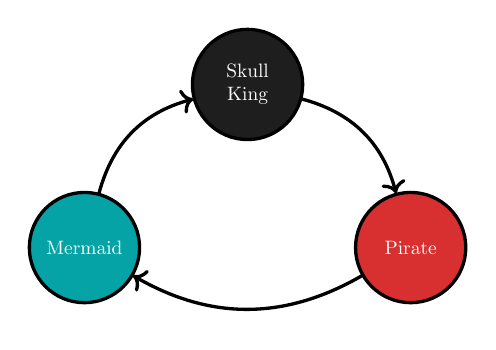
\begin{tikzpicture}[
    every node/.style={
        draw,
        circle,
        minimum size=2cm,
        inner sep=0pt,
        align=center,
        font=\normalfont,
        scale=0.7
    }, scale=0.7,
    node distance=1.5cm,
    every path/.style={line width=2mm, draw, -{Stealth[scale=1.5]}, very thick, bend left=20},
    skull/.style={fill=SkullKingBlack, text=white},
    mermaid/.style={fill=MermaidBlue, text=white},
    pirate/.style={fill=PirateRed, text=white}
]

% Nodes with colors
\node[skull] (skull) {Skull\\King};
\node[mermaid] (mermaid) [below left=of skull] {Mermaid};
\node[pirate] (pirate) [below right=of skull] {Pirate};

% Curved arrows with increased width
\draw[->] (mermaid) to[bend left=30] (skull);
\draw[->] (pirate) to[bend left=30] (mermaid);
\draw[->] (skull) to[bend left=30] (pirate);
\end{tikzpicture}

\caption{The Skull King beats the Pirate, the Pirate beats the Mermaid, and the Mermaid beats the Skull King.}
\label{trio}
\end{figure}

\subsection{Escapees}\label{escapees}
\block[]{Escapee}
If you play a Loot or Escape, you will almost never win the trick. The rare exception occurs if you start the trick with an Escapee and every one else plays an Escapee.
In that case, the first-played Escapee wins the trick.

\block{Loot}
Loot behaves just like an Escape but with one additional property: the person who plays the Loot and the person who wins the trick form an alliance. If both players' bids in
the alliance are correct at the end of the round, they each gain 20 bonus points. If either player's bid is incorrect, no bonus points are awarded.\footnote{If you start the trick with Loot and all other cards in the trick are Escapees, you would win the trick, but no alliance is formed, as you cannot form one with yourself.} Bonus points are discussed in Section~\ref{bonuses}.

\subsection{Disruptors}
\block[]{Kraken}
When this card is played, the trick is destroyed and no one wins it. The player who \textbf{would have won} the trick starts the next one.

\block{White Whale}
The White Whale destroys all Competitors (preventing them from winning) and turns all numbered cards ``white with fear,'' making them lose their suit. The player with the highest-numbered card then wins the trick (with \Black{} no longer outranking the other suits).  If more than one of the same number is present, the one played first wins.

\block{Their Ancient Feud}
If both the Kraken and White Whale are played in the same trick, the one played \textbf{second} goes into the effect, destroying the first.

\section{How they behave: suits (and leading)}
The behavior of suited cards---and, more broadly, the pattern of play for a trick---is determined by the card that \textbf{leads} the trick.
\subsection{Leading with a suit}
If the trick is led by a suited card, that suit \textbf{is set} for the rest of the trick. For subsequent players, this means
\begin{enumerate}[(a)]
\item you must play a card of the set suit \textbf{if you have one in your hand} or
\item you can play a special card (if you have one). 
\end{enumerate}
Special cards can be played at any time and do not need to follow the suits' rules.

If you \textbf{do not} have a card of the set suit in your hand, you may play any of your cards.

\block{Trick of standard suits} 
If only standard suited cards (and Escapees) are played in a trick, the highest-numbered card of the set suit wins the trick.

\block{Trump suit}
Even if the set suit is not \Black{}, a \Black{} card will beat all other suited cards.\footnote{The only way someone can play a \Black{} card if the set suit is not \Black{} is if they did not have a card of the set suit in their hand.}
Like any other suit, if there are multiple \Black{} cards in the trick (and no Competitors or Disruptors), the highest-numbered \Black{} card wins the trick.

\subsection{Leading with a special}
\block[]{Leading with a Competitor or Disruptor}
If the trick is led by a Competitor or Disruptor, \textbf{no suit is set for the remainder of the trick}.

\block{Leading with an Escapee}
If the trick is led by an Escapee, the state of the trick (whether a suit is set or not) remains undefined.
It will be determined by the first card that is not an Escapee.

\section{Bonuses}\label{bonuses}
Scores are mostly determined by whether a player's bid is correct, but there are also bonus points available. Some bonus points are ``captured'' within individual tricks, but they never contribute to the player's point total until the end of a round.

\subsection{Suited bonuses}
You'll notice that the standard suited cards with number fourteen are marked with ``+10'' and the trump suit's fourteen has ``+20.''
Whoever wins a trick that contains these cards captures the sum of the additional points indicated.

\subsection{Competitor bonuses}
There are also bonuses to be had when a competitor beats another to win a trick.
\begin{itemize}
\item 20 bonus points are captured if the Skull King defeats a Pirate,
\item 30 bonus points are captured if a Pirate defeats a Mermaid, and
\item 40 bonus points are captured if a Mermaid defeats the Skull King.
\end{itemize}
\subsection{Loot bonuses}
As mentioned in Section~\ref{escapees}, if both players in the Loot alliance make their bids, they each receieve 20 bonus points.

\section{Scoring}\label{scores}
At the end of a round, scores for each player are determined. The points you receive are a function of your bid, the number of cards dealt that round, and the number of tricks you won in the round. There are four possibilities.
\pagebreak
\begin{enumerate}[(1),listparindent=0pt]
\item If you bid 0 and your bid was correct, you gain points equal to 10 times the number of cards dealt that round.
\item If you bid 0 and your bid was incorrect, you lose points equal to 10 times the number of cards dealt that round.
\item If you bid 1 or more and your bid was correct, you gain points equal to 20 times your bid.
\item If you bid 1 or more and your bid was incorrect, you lose points equal to 10 times the ammount you were off from your bid.
\end{enumerate}

You can see from Figure~\ref{standard-payoff} that betting zero is an all-or-nothing strategy, while betting 1 or more is safer.

\begin{figure}[h]
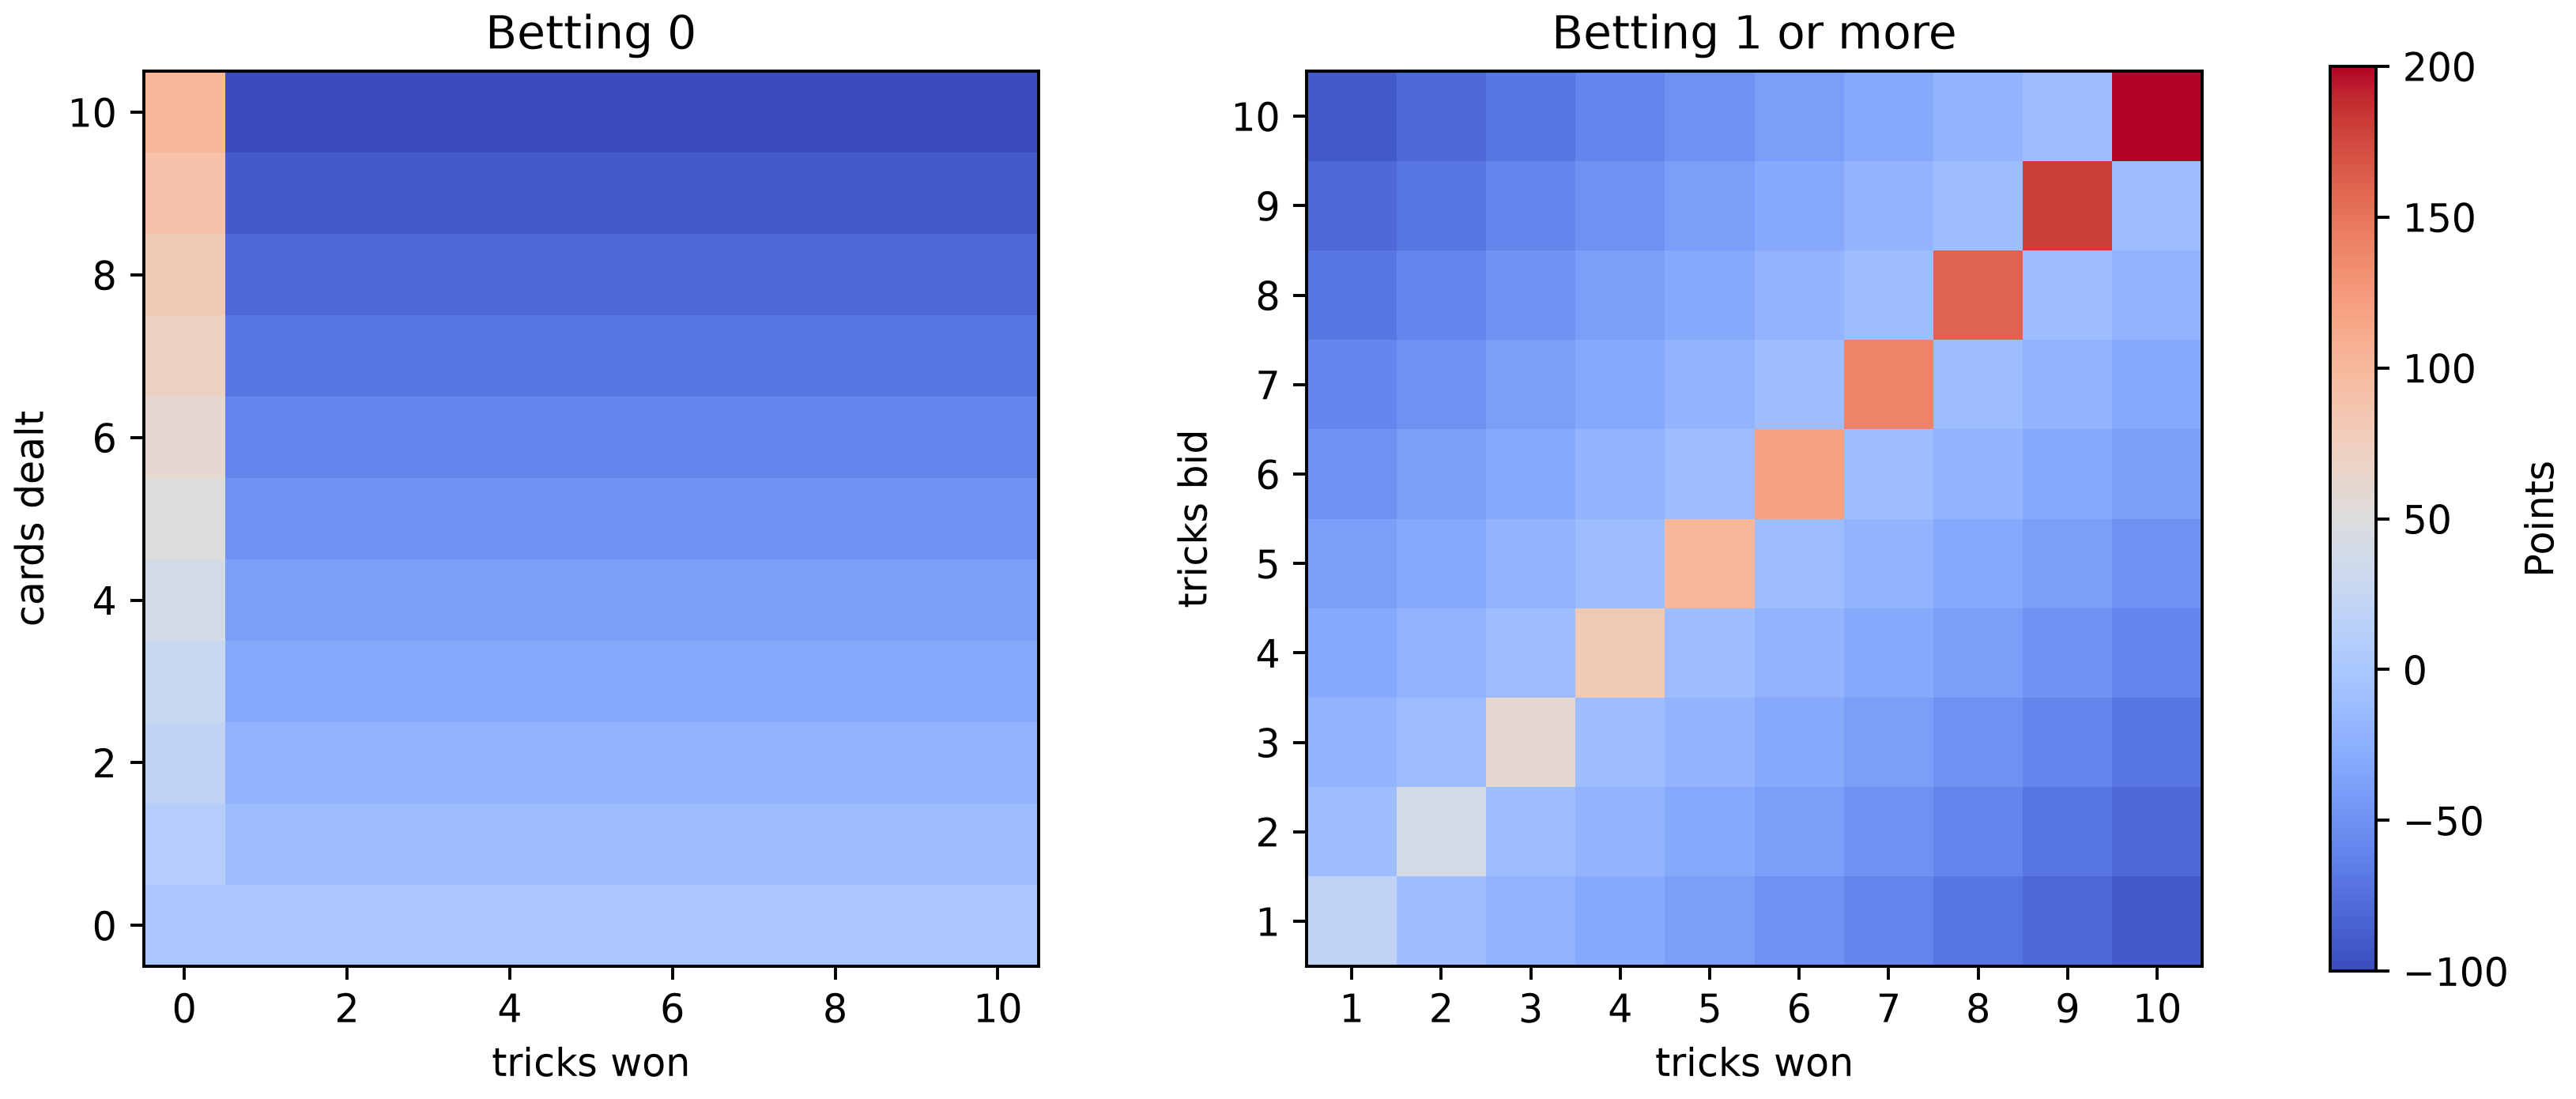
\includegraphics[width=26pc]{payoff.png}
\caption{The payoff profile for the standard rules. Notice the symmetry about the diagonal when betting 1 or more, indicating it doesn't matter if you over or under bet; you are only penalized for the absolute ammount you are off from your bid.}
\label{standard-payoff}
\end{figure}

\subsection{Bonus points}
You only earn your captured bonus points if your bid is correct.

\block{Example}
Suppose you win a trick with a \Black{} 14, \Green{} 14, and a Mermaid that beat the Skull King. Then you'd have a total of $10 + 20 + 40 = 70$ captured bonus points.

Suppose you bid three that round, but you only won two tricks. Then since you didn't make your bid, you wouldn't receive any of those bonus points, and, overall, you'd lose $10\times|2-3|=10$ points that round. But if you \textit{did} make your bid, then you'd earn $3 \times 20 + 70 = 130$ points that round---a huge payout.

\end{document}

%% For example, if five cards were dealt that round and you successfully bid 0, you would earn $5\times10 = 50$ points that round.
%% For example, if you bid 0, 7 cards were dealt that round, and your bid was incorrect, say you won 2 tricks (you could have won 5 and the loss would be the same), then you would lose $10 \times 7 = 70$ points.
%% For example, if you bid 3 and your bid was correct, you gain $20 \times 3 = 60$ points.
%% For example, if you bid 5 and you won 3 tricks, you would lose $|5 - 3| = 2 \times 10 = 20$ points. You would also lose 20 points if you won 7 tricks instead of 3, because $|5 - 7| = 2 \times 10 = 20$ points.
